\documentclass[11pt]{article}

\usepackage[margin=1in]{geometry}
\usepackage{amsmath}
\usepackage{amssymb}
\usepackage{array}
\usepackage{booktabs}
\usepackage{enumitem}
\usepackage[table]{xcolor}
\usepackage{microtype}
\usepackage{titlesec}
\usepackage{fancyhdr}
\usepackage{listings}
\usepackage{tikz}
\usetikzlibrary{arrows.meta, positioning}

% --- Colour palette ---
\definecolor{accent}{HTML}{1F4E79}
\definecolor{codebg}{HTML}{F5F7FA}
\definecolor{keep}{HTML}{2E7D32}
\definecolor{cycle}{HTML}{C62828}

% --- Section styling ---
\titleformat{\section}
  {\normalfont\large\bfseries\color{accent}}{\thesection.}{0.6em}{}[{\color{accent!40}\titlerule[1pt]}]
\titlespacing*{\section}{0pt}{1.5em}{0.6em}
\titleformat{\subsection}
  {\normalfont\bfseries\color{accent!85!black}}{\thesubsection}{0.6em}{}
\titlespacing*{\subsection}{0pt}{0.9em}{0.3em}

\renewcommand{\arraystretch}{1.25}

% --- Answer box ---
\newcommand{\answer}[1]{%
  \par\smallskip\noindent
  \fcolorbox{accent}{accent!6}{%
    \parbox{\dimexpr\linewidth-2\fboxsep-2\fboxrule\relax}{%
      \textbf{\color{accent}Result.}\ #1}}%
  \par\smallskip}

% --- Code style ---
\lstdefinestyle{py}{
  language=Python, basicstyle=\ttfamily\small, backgroundcolor=\color{codebg},
  keywordstyle=\color{accent}\bfseries, commentstyle=\color{gray}\itshape,
  stringstyle=\color{keep}, showstringspaces=false, columns=fullflexible,
  frame=single, framerule=0pt, rulecolor=\color{codebg}, xleftmargin=6pt,
  breaklines=true, aboveskip=6pt, belowskip=6pt}

\pagestyle{fancy}
\fancyhf{}
\renewcommand{\headrulewidth}{0.4pt}
\lhead{\small COMP9312 --- Project}
\rhead{\small Q1: First Cycle-Causing Edge}
\cfoot{\small\thepage}

\title{\vspace{-1.4em}\textbf{COMP9312 Project --- Q1}\\[0.2em]
\large First Cycle-Causing Edge in an Insertion Stream}
\author{YUHUI LUO \quad (z5565446)}
\date{}

\begin{document}
\maketitle
\vspace{-2.2em}

%======================================================================
\section{Problem}
We start from $n$ isolated vertices $V=\{0,1,\dots,n-1\}$ and an
\emph{undirected, unweighted} edge stream $L=[(u_1,v_1),(u_2,v_2),\dots]$, and
insert the edges one at a time. We must return the \textbf{first} inserted edge
that closes a cycle together with \textbf{one} cycle containing it, or
\texttt{None} if the stream stays acyclic. We may assume $0\le v<n$ for every
endpoint and that no edge is repeated.

%======================================================================
\section{Key Observation}
Before any cycle appears, the accepted edges form a \textbf{forest}: each kept
edge joins two vertices from \emph{different} trees and merges them. Hence an
incoming edge $(u,v)$ creates a cycle
\[
  \textbf{iff}\qquad u \text{ and } v \text{ already lie in the same tree},
\]
because that tree already contains a unique $u\!-\!v$ path and the new edge
closes it into a cycle. The task therefore reduces to \emph{maintaining
connected components under edge insertions} and, for each new edge, testing
whether its endpoints are already connected. This is precisely what a
\textbf{Disjoint Set Union} (DSU / union--find) supports.

%======================================================================
\section{Algorithm}

\paragraph{Data structures.}
\begin{itemize}[leftmargin=1.4em, itemsep=2pt]
  \item \texttt{parent[\,]}, \texttt{rank[\,]} --- DSU with \emph{path
  compression} and \emph{union by rank}.
  \item \texttt{forest[\,]} --- adjacency lists of the accepted (non-cycle)
  edges, i.e.\ the current spanning forest. It never holds more than $n-1$ edges.
\end{itemize}

\paragraph{Processing the stream.} For each edge $(u,v)$ in order:
\begin{enumerate}[leftmargin=1.6em, itemsep=2pt]
  \item If $\textsf{find}(u)=\textsf{find}(v)$, then $u,v$ are already connected:
  $(u,v)$ is the first cycle-causing edge. Recover the cycle and return.
  \item Otherwise accept it: append $(u,v)$ to \texttt{forest}, call
  $\textsf{union}(u,v)$, and continue.
\end{enumerate}
If the loop ends with no collision, return \texttt{None}.

\paragraph{Recovering the cycle.} When the collision edge $(u,v)$ is found, $u$
and $v$ are in the \emph{same} tree of the spanning forest. A single
\textbf{BFS from $u$} inside \texttt{forest} finds the unique tree path
$u\rightarrow\cdots\rightarrow v$; appending $u$ closes the cycle. We return
$\big[[u,v],\,[u,\dots,v,u]\big]$.

%----------------------------------------------------------------------
\subsection{Worked Example (spec Example~1)}
$n=6$, $L=[(0,1),(1,2),(3,4),(2,3),(4,5),(5,0)]$. The first five edges are
accepted and build the single tree $0\!-\!1\!-\!2\!-\!3\!-\!4\!-\!5$. The sixth
edge $(5,0)$ satisfies $\textsf{find}(5)=\textsf{find}(0)$ and is the first cycle
edge; BFS from $5$ reaches $0$ along $5\!-\!4\!-\!3\!-\!2\!-\!1\!-\!0$.

\begin{center}
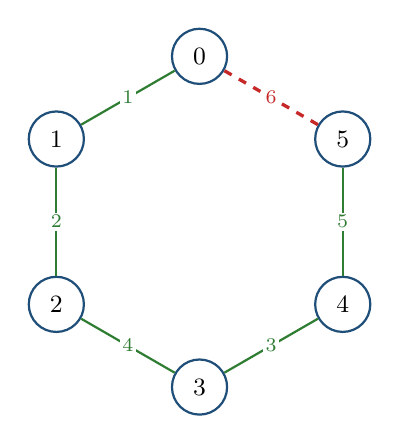
\begin{tikzpicture}[
    vtx/.style={circle, draw=accent, thick, minimum size=7mm,
      inner sep=0pt, font=\small},
    lbl/.style={midway, fill=white, inner sep=1pt, font=\scriptsize},
    keepedge/.style={keep, thick},
    cycedge/.style={cycle, very thick, dashed}]
  \foreach \i/\ang in {0/90, 1/150, 2/210, 3/270, 4/330, 5/30}
    \node[vtx] (n\i) at (\ang:2.1) {\i};
  % accepted spanning-forest edges (green) with insertion order labels
  \draw[keepedge] (n0)--(n1) node[lbl]{1};
  \draw[keepedge] (n1)--(n2) node[lbl]{2};
  \draw[keepedge] (n3)--(n4) node[lbl]{3};
  \draw[keepedge] (n2)--(n3) node[lbl]{4};
  \draw[keepedge] (n4)--(n5) node[lbl]{5};
  % cycle-causing edge (red, dashed)
  \draw[cycedge] (n5)--(n0) node[lbl]{6};
\end{tikzpicture}
\end{center}
\vspace{-0.4em}
\begin{center}\footnotesize
\textcolor{keep}{$\blacksquare$ accepted forest edges (labelled by insertion
order)} \qquad
\textcolor{cycle}{$\blacksquare$ edge 6 = $(5,0)$ closes the cycle}
\end{center}

\answer{$\big[[5,0],\ [5,4,3,2,1,0,5]\big]$}

%======================================================================
\section{Correctness}
\begin{itemize}[leftmargin=1.4em, itemsep=3pt]
  \item \textbf{First cycle detection.} By induction the accepted edges are
  always a forest, so DSU components are exactly the trees. The test
  $\textsf{find}(u)=\textsf{find}(v)$ is true \emph{iff} a $u\!-\!v$ path already
  exists, i.e.\ \emph{iff} $(u,v)$ would form a cycle. Edges are examined in
  stream order and we return on the first collision, so it is \emph{the} first
  cycle-causing edge.
  \item \textbf{Valid cycle.} At the collision the forest is not yet modified by
  $(u,v)$, so the BFS path $u\rightarrow\cdots\rightarrow v$ consists only of
  genuine earlier edges; with $(u,v)$ it forms a simple cycle containing the new
  edge.
\end{itemize}

%======================================================================
\section{Complexity Analysis}
Let $n$ be the number of vertices and $m=|L|$ the number of inserted edges.

\subsection{Time complexity: $O\big(m\cdot\alpha(n)+n\big)$}
Each edge performs two \textsf{find} operations and at most one \textsf{union}.
With path compression and union by rank, each DSU operation costs amortised
$O(\alpha(n))$, where $\alpha$ is the inverse Ackermann function
($\alpha(n)\le 4$ for all practical $n$). Over the whole stream this is
$O(m\cdot\alpha(n))$. The cycle-recovery BFS runs \emph{once}, over a forest of
at most $n-1$ edges, costing $O(n)$. Hence the total query time is
\[
  O\big(m\cdot\alpha(n)+n\big),
\]
which is effectively linear in the size of the input.

\subsection{Space complexity: $O(n)$}
\begin{itemize}[leftmargin=1.4em, itemsep=2pt]
  \item \texttt{parent[\,]} and \texttt{rank[\,]}: $O(n)$.
  \item \texttt{forest[\,]}: stores only accepted edges; a forest on $n$
  vertices has at most $n-1$ edges, so $O(n)$ --- \emph{independent of $m$}.
  \item BFS \texttt{prev} map and queue: $O(n)$.
\end{itemize}
Total working space is $O(n)$. In particular we never store the whole edge set,
only the growing spanning forest, so the data structure needed for query
processing is $O(n)$ rather than $O(n+m)$.

%======================================================================
\section{Reference Implementation}
\begin{lstlisting}[style=py]
class FirstCycleEdgeQuery:
    def query(self, n, L):
        parent = list(range(n)); rank = [0] * n
        forest = [[] for _ in range(n)]        # spanning forest (accepted edges)

        def find(x):                            # iterative path compression
            root = x
            while parent[root] != root: root = parent[root]
            while parent[x] != root: parent[x], x = root, parent[x]
            return root

        for u, v in L:
            ru, rv = find(u), find(v)
            if ru == rv:                        # u, v already connected -> cycle
                return [[u, v], self._recover_cycle(forest, u, v)]
            forest[u].append(v); forest[v].append(u)   # accept edge
            if rank[ru] < rank[rv]: ru, rv = rv, ru     # union by rank
            parent[rv] = ru
            if rank[ru] == rank[rv]: rank[ru] += 1
        return None

    def _recover_cycle(self, forest, u, v):
        from collections import deque
        prev = {u: u}; q = deque([u])
        while q:                                # BFS in the forest: u -> ... -> v
            x = q.popleft()
            if x == v: break
            for y in forest[x]:
                if y not in prev: prev[y] = x; q.append(y)
        path = [v]
        while path[-1] != u: path.append(prev[path[-1]])
        path.reverse(); path.append(u)          # [u, ..., v, u]
        return path
\end{lstlisting}

\end{document}
